\documentclass{standalone}
\usepackage{tikz}
\usetikzlibrary{arrows, positioning}

\begin{document}

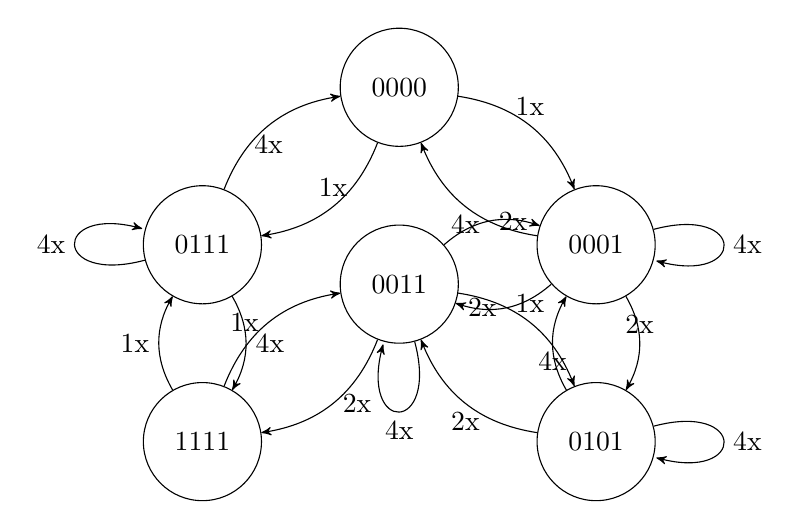
\begin{tikzpicture}[->, >=stealth', node distance=2.5cm, scale=1, every node/.style={transform shape}]

  \tikzstyle{vertex}=[circle, draw, minimum size=1.5cm]
  
  \node[vertex] (0000) {0000};
  \node[vertex] (0111) [left of=0000, yshift=-2cm] {0111};
  \node[vertex] (1111) [below of=0111] {1111};
  \node[vertex] (0011) [below of=0000] {0011};
  \node[vertex] (0001) [right of=0000, yshift=-2cm] {0001};
  \node[vertex] (0101) [below of=0001] {0101};

  \path[->] 
    (0000) edge [bend left] node[above] {1x} (0111)
    (0111) edge [bend left] node[below] {4x} (0000)
    (0000) edge [bend left] node[above] {1x} (0001)
    (0001) edge [bend left] node[below] {4x} (0000)
    (0111) edge [loop left] node[left] {4x} (0111)
    (0001) edge [loop right] node[right] {4x} (0001)
    (1111) edge [bend left] node[left] {1x} (0111)
    (0111) edge [bend left] node[right] {4x} (1111)
    (1111) edge [bend left] node[left] {1x} (0011)
    (0011) edge [bend left] node[right] {2x} (1111)
    (0001) edge [bend left] node[left] {2x} (0011)
    (0011) edge [bend left] node[right] {2x} (0001)
    (0101) edge [bend left] node[below] {4x} (0001)
    (0001) edge [bend left] node[above] {2x} (0101)
    (0101) edge [loop right] node[right] {4x} (0101)
    (0101) edge [bend left] node[below] {2x} (0011)
    (0011) edge [bend left] node[above] {1x} (0101)
    (0011) edge [loop below] node[below] {4x} (0011);

\end{tikzpicture}

\end{document}